\documentclass{article}
\usepackage{multicol}
\usepackage{amsmath}
\usepackage{graphicx}
\usepackage{float}
\usepackage{algorithm}
\usepackage{algpseudocode}
\usepackage[backend=biber]{biblatex}
\usepackage[skip=0.5em plus1pt, indent=2em]{parskip}

\setlength\columnsep{10pt}
\addbibresource{refs.bib}
%\pagenumbering{gobble}
\graphicspath{ {./figs/} }

\title{\vspace{-1cm}Volumetric Spot Noise}
\date{}
\author{Andrew Pregent}

\begin{document}
\maketitle{}
%\begin{multicols*}{2}

\section{Introduction}

In this report I will present a method of volumetric spot noise for surface texture synthesis largely based on the method by Nicolas Pavie et al. in the paper `Volumetric Spot Noise for Procedural 3D Shell Texture Synthesis' \cite{pavie:hal-02413269} with several modifications. I will then evaluate my attempts to replicate the hair and grass textures, and briefly discuss my findings extending the method to animation.

\section{Background}

% Spot noise
\par \textit{Spot noise} is a method of texture synthesis presented by Jarke J. Wijk where textures are created using a sum of impulses each convolved by a kernel function.\cite{10.1145/127719.122751}
Various textural effects can be produced by controlling the distribution of these impulses and by the type of kernel functions used.
Both ordered or stochastic effects can be achieved depending on the distributions used, and 
compared with earlier methods such as Perlin noise, spot noise has the distinct advantage of maintaining local control over the texture making it particularly versatile.

% Volumetric rendering
\par Spot noise as described by Jarke J. Wijk was purely two-dimensional, however the concept can be extended to the third dimension. Note that we can assume that kernels only affect a small neighborhood around each impulse's position. This allows us to treat the textures as sparse volumetric data, only storing the set of impulses rather than explicitly storing the texture which would be prohibitive on memory. This has the added advantage of the resulting texture being resolution independent.

There are many ways to render sparse volumetric data. One straightforward method would be to ray trace a shell mesh surrounding the texture, where rays are cast from the camera origin through each pixel and into the scene and samples are then accumulated at points along each ray. Unfortunately this means we must sample our entire volume multiple times per pixel.

%% Slicing
%Slicing attempts to speed this process up by reducing the amount of sampling required.
%We can splat each point once onto each slice and combine the slices together.
%Volumetric data can quickly become infeasible for larger or higher resolution textures.
%We can reduce the memory by only using a single slice and accumulating one at a time, but this removes an opportunity for parallelism.

% EWA splatting
\textit{EWA splatting} is a technique due to Matthias Zwicker et al. for rendering point cloud surfaces efficiently.\cite{10.1109/TVCG.2002.1021576} Their method uses three dimensional Gaussian functions as the kernel of choice for rendering impulses since they are closed under linear transformations and have a closed form solution to integration along an axis, which results in a two dimensional Gaussian. This allows us to find an approximate analytic solution for the screen-space projection of the kernels for a given view. This is much faster than raytracing since we only need to splat each kernel once, accumulating the results to a single buffer. Note however that this can only be an approximation because the perspective divide is not a linear operation.

% Transparency and OI
Note that the set of impulses must be ordered with respect to their depth from the camera if we wish to use translucent kernels with traditional methods of blending. Since the camera typically moves per-frame, this means the impulses must also be sorted per-frame which can be computationally prohibitive with large sets of impulses.

Morgan McGuire and Louis Bavoil propose a method of \textit{depth weighted order independent transparency} for rendering transparent objects in a scene by weighting the kernels according to their depth from the camera.\cite{McGuire2013Transparency}
In addition to allowing us to continue to use the more efficient EWA splatting, this also avoids an artifact known as popping which can be an issue with sorting based methods.

\section{Method}

\subsection{Initialization}

The process of texture generation begins by creating a set of impulses. Each has a position, orientation, and color associated with it. Our goal is to place these kernels close to the surface of the input mesh, and to be able to associate their parameters with points on the surface of the mesh.

One simple method which can yield acceptable results for sparse textures is to simply iterate the faces of the mesh. This can partially solved by adjusting how many impulses to place per face based upon the area of the faces. However for wildly varying face sizes or for dense textures another approach is needed, otherwise the structure of the underlying mesh will become apparent.

An octree is suggested by Pavie et al. for this purpose. The leaf nodes were each assigned a certain number of impulses which could be projected onto a planar approximation of the surface using the surface normal of a face nearest the center of the leaf node.
Each leaf node must be small enough that the linear approximation is sufficient, so for manifolds of high curvature this will be a slow process.

Note that the actual octree is purely conceptual and does not have to be stored, only the set of impulses is needed for later steps. See Algorithm \ref{alg:init} for a sketch of the algorithm.

\begin{algorithm}
\caption{Initialization} \label{alg:init}
\begin{algorithmic}
\State Let ${pending}$ be a new queue
\State Push minimum axis aligned cube which bounds ${mesh}$ to ${pending}$
\While{$|{pending}| \neq 0$}
\State ${top} \gets \text{pop}({pending})$
\If{$\text{width}({top}) \leq \text{limit}$}
\State Get nearest point and surface normal to $\text{center}({top})$ in mesh
\State Pick random point(s) in ${top}$ and project onto plane
\Else
\State Bisect ${top}$ along center of all three axes
\State Push each resulting cube which intersects ${mesh}$ to ${pending}$
\EndIf
\EndWhile
\end{algorithmic}
\end{algorithm}

\subsection{EWA Splatting}

The EWA splatting method which was used and will be described in this section is the two dimensional kernel approximation due to Matthias Zwicker et al. rather than the hybrid raymarching approach suggested by Pavie et al.\cite{10.1109/TVCG.2002.1021576}\cite{pavie:hal-02413269} This was chosen because of its computational efficiency, while yielding comparable results.

Recall that our kernel is a three-dimensional Gaussian of the form:

\begin{align}
K(x;x_0) = \frac{\exp\left({-\frac{1}{2}(x-x_0)^T\Sigma^{-1}(x-x_0)}\right)}{\sqrt{(2\pi)^3|\Sigma|}}
\end{align}

Where $x_0$ is the center of each impulse and $\Sigma=RSS^TR^T$ where $R$ is the orientation and $S$ the scale of our impulse.

Now we transform from world to camera coordinates. The position $x_0$ will be transformed separately, for now we focus on the orientation and scale of the new kernel.

\begin{align}
\Sigma' = JW_{3\times 3} \; \Sigma \; W_{3\times 3}^TJ^T
\end{align}

Here $W_{3\times 3}$ is the rotational component of the transformation from world to camera coordinates and $J$ is the Jacobian matrix of the approximation of the perspective divide. To transform from camera coordinates to screen coordinates we need to perform what is known as a perspective divide but this is a non-linear operation which usually involves dividing the homogeneous coordinates by their last coordinate. Since this is not a linear operation the resulting function would no longer be Gaussian.

To work around this we can use an affine approximation of the perspective divide. Let $m$ take the points from camera space to screen space.

\begin{align}
m = \left[
\begin{array}{ccc}
x_1/x_3 \\
x_2/x_3 \\
|x| \\
\end{array}
\right]
\end{align}

We can approximate this with the first two terms of the Taylor series as $m(x_0)+\frac{\partial m}{\partial x}(x-x_0)$ where $J$ is the Jacobian of $m$ given below.

\begin{align}
J = \frac{\partial m}{\partial x} = \left[
\begin{array}{ccc}
    1/x_3   &        0 &  -x_1/x_3^2 \\
    0       &    1/x_3 &  -x_2/x_3^2 \\
    x_1/|x| &  x_2/|x| &   x_3/|x|   \\
\end{array}
\right]
\end{align}


The transformed two dimensional Gaussian becomes:

\begin{align} \label{eq:1}
K'(x';x_0') = \frac{ \exp\left(-\frac{1}{2}{(x'-x_0')^T(\Sigma'_{2\times 2})^{-1}(x'-x_0')}\right) }{2\pi\sqrt{|\Sigma'_{2\times 2}|}}
\end{align}

Where $\Sigma'_{2\times 2}$ is the top left $2\times 2$ partition of $\Sigma$ and $x_0'$ is the transformed impulse center (such that $x_0'=Wx_0$).

To avoid aliasing this function is convolved with a low pass filter $h$ - another Gaussian function. This has the effect of softening the output, particularly at the edges. This amounts to adding the filter's variance matrix (the identity matrix multiplied by some constant factor $\lambda$) to $\Sigma'_{2\times 2}$ before inversion in equation \ref{eq:1}.

The final two dimensional Gaussian with low-pass filter is:

\begin{align} \label{eq:2}
K'(x';x_0')\circ h = \frac{ \exp\left(-\frac{1}{2}{(x'-x_0')^T(\Sigma'_{2\times 2} + \lambda I)^{-1}(x'-x_0')}\right) }{2\pi\sqrt{|\Sigma'_{2\times 2}|}}
\end{align}

\subsection{Order Independent Transparency}

The traditional method of blending uses a simple linear interpolation between the current color value and the color value being blended over top, which can be represented as the recurrance relation in Equation \ref{eq:blend}.

\begin{align} \label{eq:blend}
C_{n+1} = \alpha_{n+1} c_{n+1} + (1-\alpha_{n+1}) C_{n}
\end{align}

This operation is highly order dependent: the colors blended later generally have a much larger effect on the final color. For this reason the traditional alpha blending method involves sorting by depth each frame, so that the objects nearer to the camera have a greater visual effect on the final color.

This means that we can use depth as a heuristic in approximating the effect which a given color will have on the final color at each pixel. Since the distribution of depth values in a scene is often not uniform this means we must tailor our approximation to the nature of an individual scene.

Morgan McGuire and Louis Bavoil suggest the following function to approximate blending.\cite{McGuire2013Transparency}

\begin{align} \label{eq:wblend}
C_f \approx \frac{\sum\limits^n_{i=1} w_iC_i}{\sum\limits^n_{i=1} w_i\alpha_i}
    \left[ 1-\prod_{i=1}^n{(1-\alpha_i)} \right] + C_0\prod_{i=1}^n{(1-\alpha_i)}
\end{align}

The weight factor must be chosen carefully depending on the effect desired. For example for the hair in this report the following hybrid weight function was used which uses both depth and the color itself, due to Morgan McGuire.\cite{mcguire_2014}

\begin{align} \label{eq:3}
w_i = \text{clamp}(\alpha\text{max}\{r, g, b\}, \alpha, 1) \cdot
    \text{clamp}\left(\frac{0.03}{10^{-5} + (z / 200)^4}, 0.01, 3\times10^3\right)
\end{align}

Where $\alpha$ is is the transparency of the material multiplied by the result of Equation \ref{eq:2}, $r,g,b$ are the color values of the material and $z$ is the depth of the impulse in screen space.

The following pseudocode summarizes the process of rendering a frame using weighted blending. 

\begin{algorithm}
\caption{Frame drawing} \label{alg:wblend}
\begin{algorithmic}
\State Enable depth write and depth test
\State Render solid geometry to depth buffer.
\State Disable depth write, enable depth test \Comment{Culls splats behind solid geometry}
\State Splat EWA kernels using Equation \ref{eq:2}
\State Disable depth test
\State Compose results using Equation \ref{eq:3}
\end{algorithmic}
\end{algorithm}

\section{Results}

\begin{figure*}
    \vspace{-1cm}
     \makebox[\textwidth][c]{
        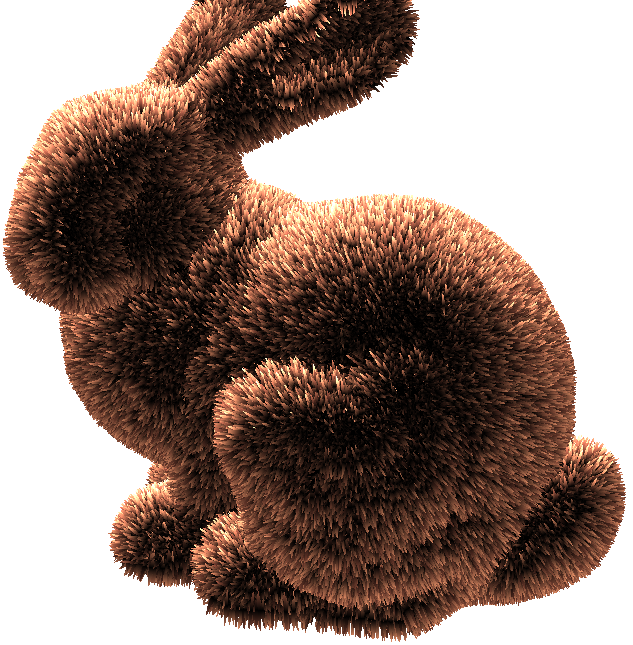
\includegraphics[width=10cm]{hair8}
        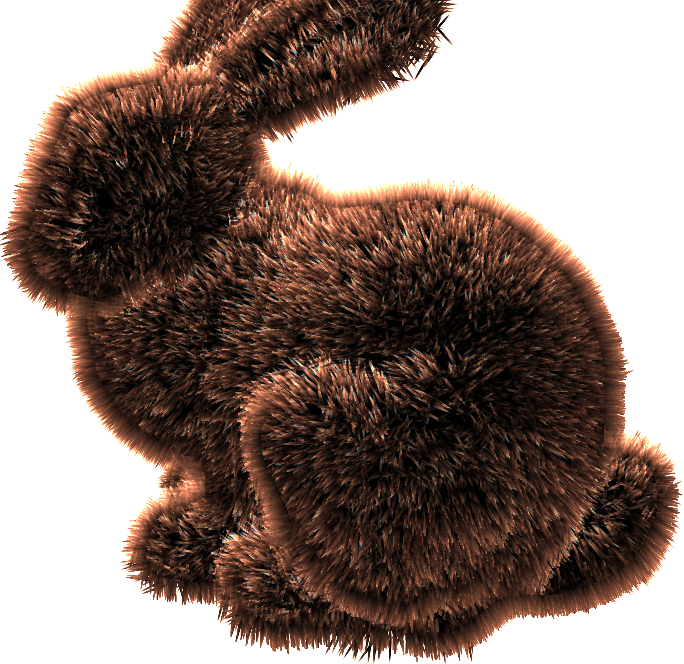
\includegraphics[width=10cm]{hair10}
     }\\
     \makebox[\textwidth][c]{
        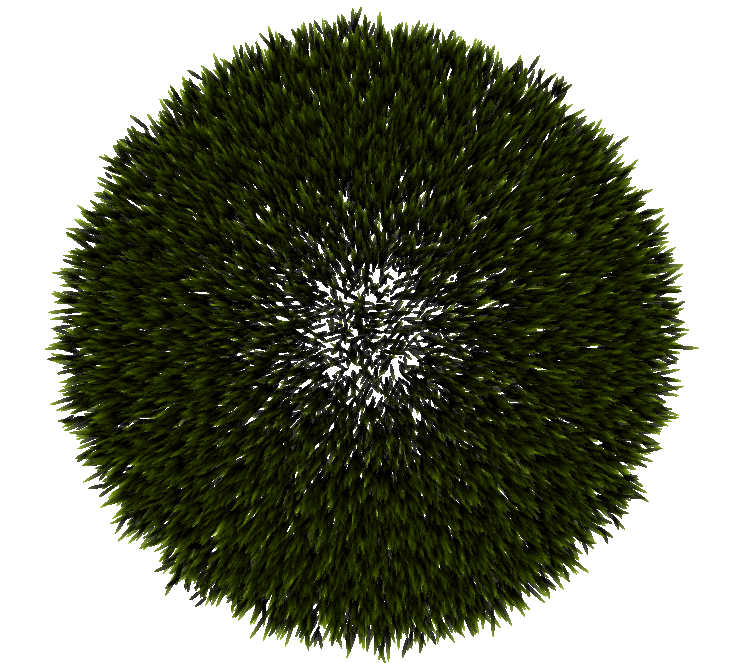
\includegraphics[width=10cm]{grass}
        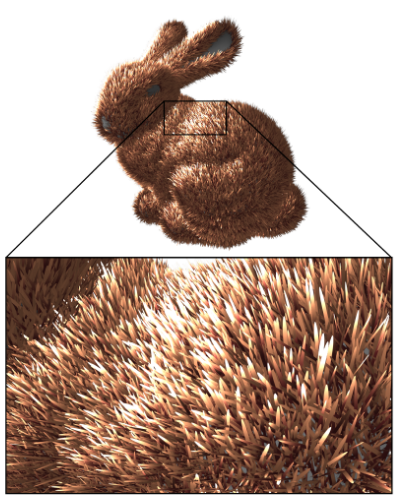
\includegraphics[width=5cm]{paperhair}
        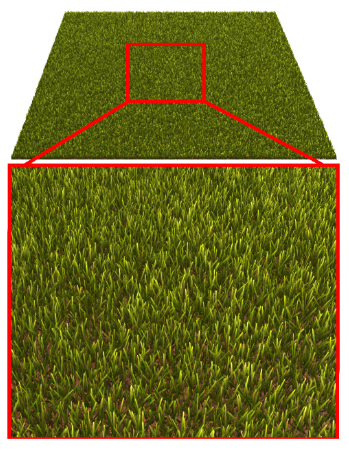
\includegraphics[width=5cm]{papergrass}
     }
    \caption{Hair rendering without (\textit{top left}) and with (\textit{top right}) order independent transparency. \textit{Bottom left: } Grass hill rendered from above. \textit{Bottom right:} Results of Pavie et al.}
    \label{fig:strand}
    \end{figure*}

I will now present the results of my implementation. I was particularly interested in trying to replicate the results of the hair and grass textures by Pavie et al, and so this is what I will focus on and compare against.

The both hair and grass textures were created by using long thin translucent Gaussian kernels. The long axis of each kernel was transformed to camera space and used to add a color gradient so that the roots of each strand were darker - simulating the effect of strands occluding eachother from light nearer to the mesh's surface. For the hair example each strand was also flat shaded. Hair direction mostly followed the surface normal with slight random variation. Adding a manual bias to the hair direction would be a source for future improvement as it would better cover the underlying mesh.

One issue observed when using order independent transparency is that lighter bands or `halos' tend to be present around the objects due to the large amount of blending in these areas (see Figure \ref{fig:strand}). This could potentially be solved by further adjusting the weight function used for blending.

Finally, because of the control offered by interpolating the impulse distributions, the method extends naturally to animation. In the hair and grass examples a wind rippling effect was achieved by rotating the impulses along an axis perpendicular to the major axis by a function which varied over time. I also found that skewing the variance matrix instead of rotating had an interesting effect which could be used instead depending on the texture and effect desired.

\begin{align} \label{eq:anim}
    f(t;x) = \frac12\cos\left(5(x_1-x_2-x_3-\frac12\cos(t)-t)\right)
\end{align}

Equation \ref{eq:anim} is illustrative of the types of functions which were used to control the animation. I found that oscillations which combined both the spatial and time domains worked well to create a ripple effect, and that by nesting trigonometric functions I could oscillate the speed of oscillations which helped to produce a natural looking result. Here $t$ increased over time and $x$ was the center of each impulse.


\section{Conclusion}

In this report I have shown a method based on the work of Nicolas Pavie et al. for synthesizing surface textures using volumetric spot noise. The method has been modified to use the two dimensional kernel by Matthias Zwicker et al. An application of the method to animated textures has also been provided.

As a method for creating strand based textures such as grass and hair I believe that compelling visual results can be achieved. However there are significant downsides to this method which limit its use. Since the graphics pipeline is adapted for more traditional polygonal based approaches these have a speed advantage over splatting based methods.
When compared with curve based approaches the method currently lacks a direct way to bend individual strands. Using several kernels for each strand might address this, however preliminary tests suggest that making the transition between kernels seamless would be difficult, especially for animation.

This method does however still present several advantages. Depth weighted transparency does not suffer the same `popping' artifacts during animation that the common shell based method might. The method is also well suited to handle the translucent effect present in hair and foilage, as well as to add subtle blur with the low-pass filter that would be much more difficult to achieve using a polygonal technique.

I believe future work could be done to combine the advantages of this method such as the low-pass filter and weighted order independent transparency with a more traditional curve based approach.

\printbibliography{}
%\end{multicols*}
\end{document}